% ------------------------------------------------------------------------------
% TYPO3 Version 10.1 - What's New (Dutch Version)
%
% @license	Creative Commons BY-NC-SA 3.0
% @link		http://typo3.org/download/release-notes/whats-new/
% @language	Dutch
% ------------------------------------------------------------------------------

\section{Wijzigingen voor Integrators}
\begin{frame}[fragile]
	\frametitle{Wijzigingen voor Integrators}

	\begin{center}\huge{Hoofdstuk 2:}\end{center}
	\begin{center}\huge{\color{typo3darkgrey}\textbf{Wijzigingen voor Integrators}}\end{center}

\end{frame}

% ------------------------------------------------------------------------------
% Feature | 89102 | Read settings for sites from <config>/sites/<siteIdentifier>/settings.yaml
%
%\begin{frame}[fragile]
%	\frametitle{Wijzigingen voor Integrators}
%	\framesubtitle{Site-specific Settings (1)}
%
%	% decrease font size for code listing
%	\lstset{basicstyle=\smaller\ttfamily}
%
%	\begin{itemize}
%		\item A YAML file can provide site specific variables independent of the current context.
%
%		\item Place the file in the site configuration folder:\newline
%			\texttt{<config>/sites/<siteIdentifier>/settings.yaml}
%
%		\item For example:
%
%\begin{lstlisting}
%Vendor:
%   MyExtension:
%      storagePid: 1
%      limit: 15
%\end{lstlisting}
%
%	\end{itemize}
%
%\end{frame}
%
% ------------------------------------------------------------------------------
% Feature | 89102 | Read settings for sites from <config>/sites/<siteIdentifier>/settings.yaml
%
%\begin{frame}[fragile]
%	\frametitle{Wijzigingen voor Integrators}
%	\framesubtitle{Site-specific Settings (2)}
%
%	% decrease font size for code listing
%	\lstset{basicstyle=\smaller\ttfamily}
%
%	\begin{itemize}
%		\item Settings can be accessed in TypoScript:
%
%\begin{lstlisting}
%plugin.tx_example.storagePid = {$Vendor.MyExtension.storagePid}
%\end{lstlisting}
%
%		\item Settings can also be accessed in PHP using the \texttt{Site} object:
%
%\begin{lstlisting}
%$settings = $site->getSettings();
%$storagePid = $settings['MyVendor']['MyExtension']['storagePid'];
%\end{lstlisting}
%
%	\end{itemize}
%
%\end{frame}

% ------------------------------------------------------------------------------
% Feature | 89227 | Ask for email address while installing TYPO3

\begin{frame}[fragile]
	\frametitle{Wijzigingen voor Integrators}
	\framesubtitle{E-mailadres beheerder}

	\begin{columns}[T]
		\begin{column}{.04\textwidth}
		\end{column}
		\begin{column}{.38\textwidth}

			Een e-mailadres kan nu ingevuld worden tijdens het installatieproces.
			Dit adres wordt gebruikt voor de backendgebruiker van de eerste beheerder.

			\vspace{0.2cm}

			Dezelfde optie is aanwezig in de Onderhoudsmodule van de Install Tool
			\textbf{Beheerder aanmaken}.

		\end{column}
		\begin{column}{.58\textwidth}
			\vspace{-0.3cm}
			\begin{figure}
				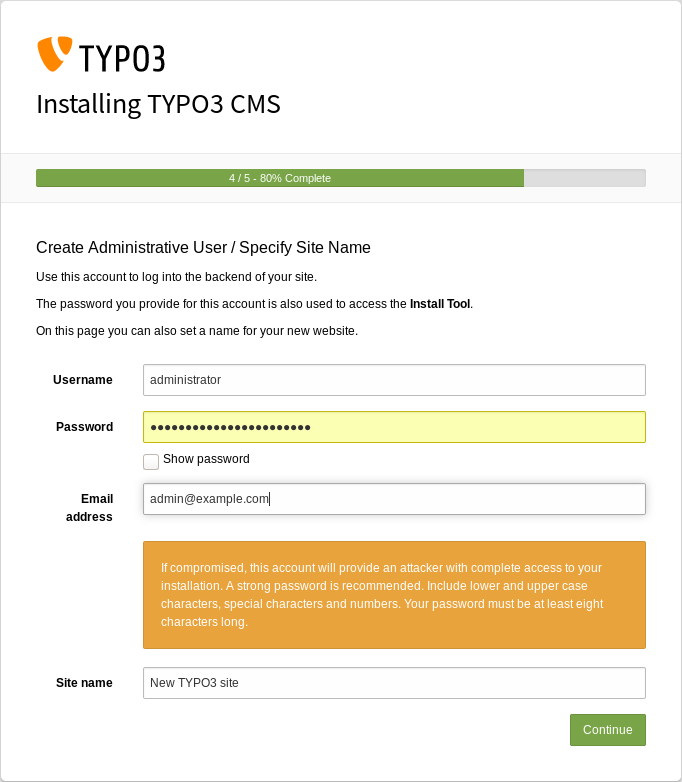
\includegraphics[width=0.70\linewidth]{ChangesForIntegrators/89227-EmailAddressDuringInstallation.png}
			\end{figure}
		\end{column}
	\end{columns}

\end{frame}

% ------------------------------------------------------------------------------
% Feature | 89229 | Cache Preset for Settings in Maintenance Area

% TRANSLATORS, PLEASE BE AWARE:
% We already included this slide in the 10.0 What's New Slides! However, the
% feature #89229 was removed from the TYPO3 core shortly before version 10.0 was
% published. Therefore, you possibly don't need to translate this slide again
% (just copy the text from the previous What's New Slides (search for the term
% "Cache Storage Type" in file ChangesForIntegrators.tex).

\begin{frame}[fragile]
	\frametitle{Wijzigingen voor Integrators}
	\framesubtitle{Soort cacheopslag (1)}

	\begin{itemize}

		\item TYPO3 biedt een flexibel cachesysteem met een standaardconfiguratie
			die perfect is voor de meeste gevallen.
		\item Het type opslage kan nu geconfigureerd worden om de caches af te regelen en
			de prestaties te verbeteren, afhankelijk van de eigen omgeving.

			\begin{itemize}
				\item Kies de \textbf{database}-opslag voor een standaardomgeving
					of als er een netwerkbestandssysteem (NFS) bijvoorbeeld gebruikt wordt.
				\item Kies het \textbf{bestandssysteem} als een gedistribueerde database
					bijvoorbeeld gebruikt wordt.
				\item Kies \textbf{aangepaste cache-instellingen} om het opslagtype
					voor elke cache apart te configureren.
			\end{itemize}

		\item Voor meer complexe installaties zouden geheugengebaseerde caches zoals
			\href{https://redis.io/}{Redis}
			of
			\href{https://memcached.org/}{Memcached}
			overwogen moeten worden.

	\end{itemize}

\end{frame}

% ------------------------------------------------------------------------------
% Feature | 89229 | Cache Preset for Settings in Maintenance Area

% TRANSLATORS, PLEASE BE AWARE:
% We already included this slide in the 10.0 What's New Slides! However, the
% feature #89229 was removed from the TYPO3 core shortly before version 10.0 was
% published.
%
% On this slide, the path to the function in the backend needs to be adjusted:
% ADMIN TOOLS -> Settings -> Configuration Presets

\begin{frame}[fragile]
	\frametitle{Wijzigingen voor Integrators}
	\framesubtitle{Soort cacheopslag (2)}

	\begin{itemize}

		\item Backend: \textbf{ADMIN TOOLS} \ding{223}\hspace{0.1cm}\textbf{Settings} \ding{223}\hspace{0.1cm}\textbf{Configuration Presets}:
		\end{itemize}

	\begin{figure}
		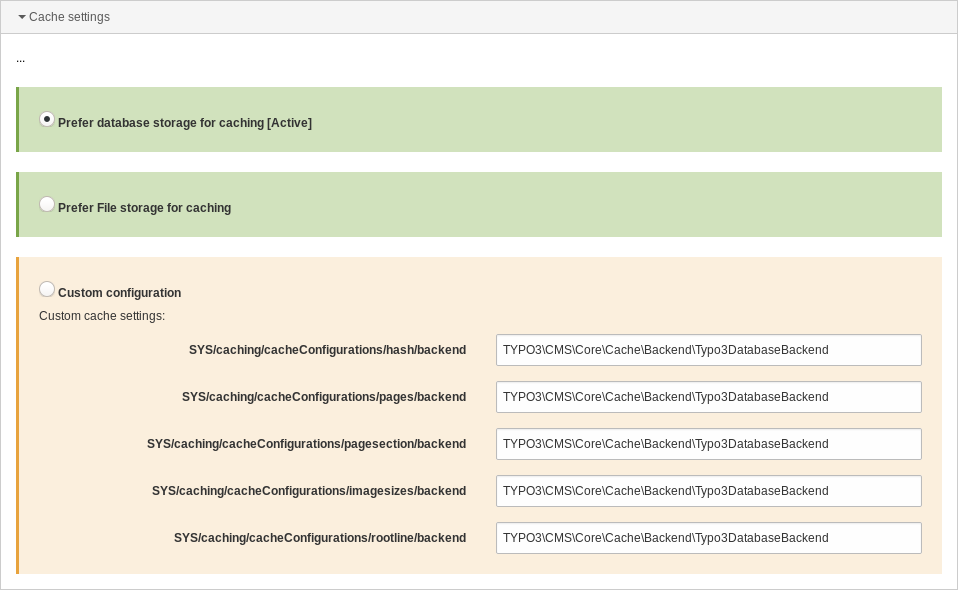
\includegraphics[width=0.60\linewidth]{ChangesForIntegrators/89229-CachePresetForSettingsInMaintenanceArea.png}
	\end{figure}

\end{frame}

% ------------------------------------------------------------------------------
% Feature | 89142 | Create site configuration if page is created on root level

\begin{frame}[fragile]
	\frametitle{Wijzigingen voor Integrators}
	\framesubtitle{Site-configuratie}

	\begin{itemize}
		\item Als een nieuwe pagina op het rootniveau wordt aangemaakt wordt een
			standaar siteconfiguratie automatisch gegenereerd.
		\item Dit maakt dat een basis TYPO3-site snel opgezet kan worden.
		\item De siteconfiguratiefuncties:

			\begin{itemize}
				\item een voorgedefinieerde identifier (bijv. \texttt{site-42-a1d0c6e83f})
				\item een beginpunt (bijv. \texttt{https://example.com/site-42})
				\item een standaardtaal (bijv. \texttt{English})
			\end{itemize}

	\end{itemize}

\end{frame}

% ------------------------------------------------------------------------------
% Feature | 89090 | Reports for conflicting redirects

\begin{frame}[fragile]
	\frametitle{Wijzigingen voor Integrators}
	\framesubtitle{Conflicterende doorverwijzingen (1)}

	\begin{itemize}
		\item Er is een nieuw Symfony commando om doorverwijzingen te detecteren
			die conflicteren met pagina-URL's.
		\item Voer het commando uit op de commandoregel:\newline
			\smaller
				(optionele parameter \texttt{-}\texttt{-site} beperkt de controle tot een specifieke site)
			\normalsize
	\end{itemize}

	\begin{figure}
		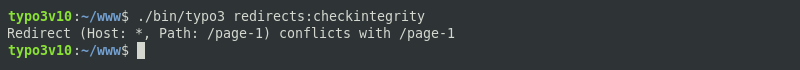
\includegraphics[width=0.90\linewidth]{ChangesForIntegrators/89090a-ReportsForConflictingRedirects.png}
	\end{figure}

	\begin{itemize}
		\item Het commando is ook beschikbaar als een taakplannertaak:
	\end{itemize}

	\begin{figure}
		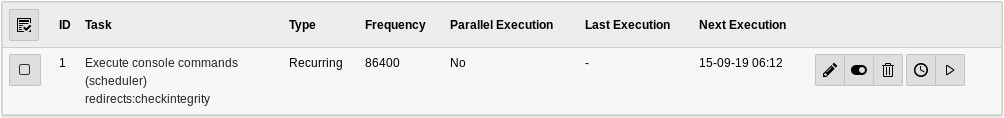
\includegraphics[width=0.90\linewidth]{ChangesForIntegrators/89090b-ReportsForConflictingRedirects.png}
	\end{figure}

\end{frame}

% ------------------------------------------------------------------------------
% Feature | 89090 | Reports for conflicting redirects

\begin{frame}[fragile]
	\frametitle{Wijzigingen voor Integrators}
	\framesubtitle{Conflicterende doorverwijzingen (2)}

	\begin{itemize}
		\item Een lijst met gevonden conflicterende doorverwijzingen is ook te vinden in de module Rapportage:
	\end{itemize}

	\begin{figure}
		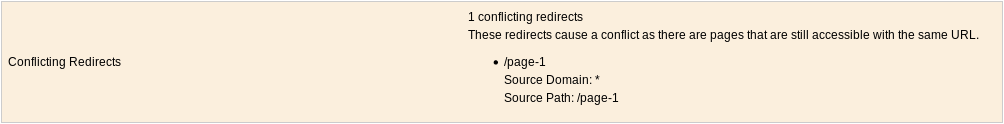
\includegraphics[width=0.90\linewidth]{ChangesForIntegrators/89090c-ReportsForConflictingRedirects.png}
	\end{figure}

	\begin{itemize}
		\item
			\small\textbf{Let op:}
				Het commando moet weer uitgevoerd worden om de lijst te "herbouwen".
				Het oplossen van het probleem (bijv. de doorverwijzing verwijderen) maakt de lijst niet leeg.
			\normalsize
	\end{itemize}

\end{frame}

% ------------------------------------------------------------------------------
% Feature | 89010 | Introduce Site Configuration for Distribution Packages

\begin{frame}[fragile]
	\frametitle{Wijzigingen voor Integrators}
	\framesubtitle{Distributiepakketten}

	% decrease font size for code listing
	\lstset{basicstyle=\tiny\ttfamily}

	\begin{itemize}
		\item Distributies kunnen nu een siteconfguratie bestand(en) bevatten.

		\item Maak een map/bestand in het distributiepakket aan als volgt:\newline
			\texttt{Initialisation/Site/<siteIdentifier>/config.yaml}

		\item Net zoals met bestanden die verplaatst worden naar \texttt{fileadmin/},\newline
			wordt siteconfiguratie verplaatst naar de map \texttt{config/}.

		\item Als de doelmap al bestaat wordt de bestaande configuratie niet gewijzigd.
	\end{itemize}

\end{frame}

% ------------------------------------------------------------------------------
% Feature | 88318 | Display Application Context in CLI

\begin{frame}[fragile]
	\frametitle{Wijzigingen voor Integrators}
	\framesubtitle{Applicatiecontext in CLI}

	\begin{itemize}
		\item De huidige applicatiecontext wordt nu getoond naast het
			TYPO3 versienummer op de opdrachtregel:
	\end{itemize}

	\begin{figure}
		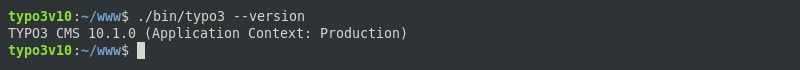
\includegraphics[width=0.90\linewidth]{ChangesForIntegrators/88318-DisplayApplicationContextInCli.png}
	\end{figure}

\end{frame}

% ------------------------------------------------------------------------------
% Feature | 87525 | Add api=1 option in VimeoRenderer

\begin{frame}[fragile]
	\frametitle{Wijzigingen voor Integrators}
	\framesubtitle{Vimeo Video Weergave}

	% decrease font size for code listing
	\lstset{basicstyle=\smaller\ttfamily}

	\begin{itemize}
		\item De parameter \texttt{api=1} in Vimeo video URL's maakt API-interactie met de videospeler
		(bijv. extra knoppen om de video te bedienen) mogelijk.
		\item Integrators kunnen deze parameter op twee manieren instellen.

		\begin{itemize}
			\item Met TypoScript:

\begin{lstlisting}
lib.contentElement.settings.media.additionalConfig.api = 1
\end{lstlisting}

			\item In Fluid met de Media-ViewHelper:

\begin{lstlisting}
<f:media
  file="{file}"
  alt="{file.properties.alternative}"
  title="{file.properties.title}"
  additionalConfig="{api: 1}"
/>
\end{lstlisting}

		\end{itemize}
	\end{itemize}

\end{frame}

% ------------------------------------------------------------------------------
% Feature | 86670 | Make default action in DragUploader adjustable

\begin{frame}[fragile]
	\frametitle{Wijzigingen voor Integrators}
	\framesubtitle{Bestandsuploads}

	% decrease font size for code listing
	\lstset{basicstyle=\smaller\ttfamily}

	\begin{itemize}
		\item De standaardactie bij het uploaden van bestanden via verslepen in de bestandslijst module kan nu ingesteld worden.
		\item User TSConfig:

\begin{lstlisting}
# Standaard vervangen:
options.file_list.uploader.defaultAction = replace

# Standaard hernoemen:
options.file_list.uploader.defaultAction = rename

# Standaard annuleren:
options.file_list.uploader.defaultAction = cancel
\end{lstlisting}

	\end{itemize}

\end{frame}

% ------------------------------------------------------------------------------
% Feature | 84250 | Separately enable / disable "Add media by URL" and "Select & upload files"

\begin{frame}[fragile]
	\frametitle{Wijzigingen voor Integrators}
	\framesubtitle{Media-elementknoppen}

	% decrease font size for code listing
	\lstset{basicstyle=\tiny\ttfamily}

	\begin{itemize}
		\item Knoppen \textbf{"Media toevoegen op URL"} en \textbf{"Kiezen \& bestanden uploaden"}
			kunnen nu onafhankelijk van elkaar in-/uitgeschakeld worden.
	\end{itemize}

	\begin{figure}
		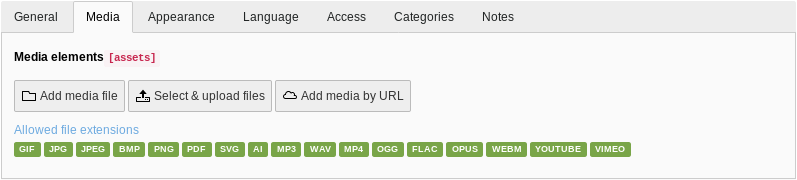
\includegraphics[width=0.75\linewidth]{ChangesForIntegrators/84250-EnableDisableMediaButtons.png}
	\end{figure}

	\begin{itemize}
		\item Dit voorbeeld verbergt beide knoppen:

\begin{lstlisting}
$GLOBALS['TCA']['pages']['columns']['media']['config']['appearance'] = [
  'fileUploadAllowed' => false,
  'fileByUrlAllowed' => false,
];
\end{lstlisting}

	\end{itemize}

\end{frame}

% ------------------------------------------------------------------------------
% Feature | 88441 | Show configuration of USER_INT objects in adminpanel

\begin{frame}[fragile]
	\frametitle{Wijzigingen voor Integrators}
	\framesubtitle{Admin-paneel}

	\begin{itemize}
		\item Het admin-paneel heeft een nieuw onderdeel \textbf{USER\_INT} in de "Info" module.
	\end{itemize}

	\begin{figure}
		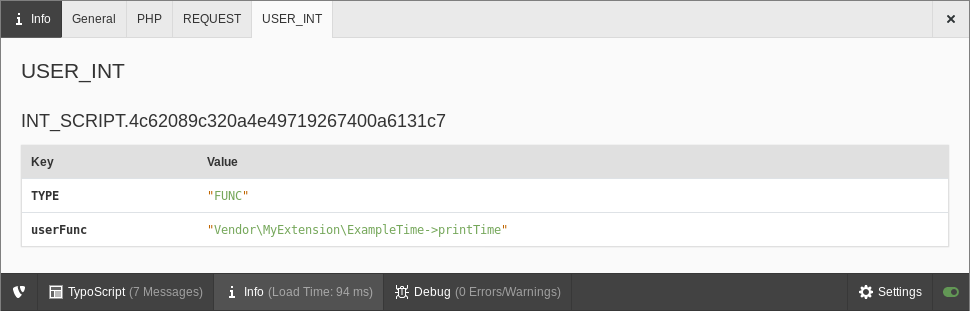
\includegraphics[width=0.90\linewidth]{ChangesForIntegrators/88441-ShowUserIntObjectsInAdminPanel.png}
	\end{figure}

\end{frame}

% ------------------------------------------------------------------------------
